% LTeX: language=de-DE
\section{Virtuelle Maschine}

\begin{frame}{Virtuelle Maschine}
	\begin{itemize}
		\item Oft: Eine \emph{Virtuelle Maschine} (VM) simuliert echte Computer
		      \begin{itemize}
			      \item Display
			      \item Lautsprecher
			      \item Festplatte
			      \item \dots
		      \end{itemize}
		\item Hier: Software, die wie die CPU eines Rechners funktioniert
	\end{itemize}
\end{frame}

\begin{frame}{Wie eine CPU Programme ausführt \TODO{DELETE}}
	\begin{itemize}
		\item Die meisten Prozessoren basieren auf der \emph{von Neumann Architektur}~\scite[p.~172]{Ledin2020-yp}
		\item Eine CPU enthält nach von Neumann ein \emph{Rechenwerk}\footnote{Engl: \enquote{arithmetic logic unit} (ALU).}, \emph{Steuerwerk}\footnote{Engl: \enquote{control unit}.}, \emph{Speicherwerk}, \emph{Ein- / Ausgabewerk} und ein Bussystem~\scite[p.~172]{Ledin2020-yp}
		\item Die Programmausführung wird durch den sog. \emph{Befehlszyklus}\footnote{Engl: \enquote{fetch-decode-execute cycle}.} modelliert~\scite[pp.~208-209]{Ledin2020-yp}:
		\item[] \begin{enumerate}
				\item \textbf{Fetch} (Befehl laden): Das Steuerwerk lädt die nächste Anweisung aus dem Speicher
				\item \textbf{Decode} (Befehl dekodieren): Der Befehlscode und die Operanden werden ermittelt
				\item \textbf{Execute} (Befehl ausführen): Die zuständige Einheit im Prozessor wird verwendet, um den Befehl zu verarbeiten.
				      Beispielsweis wird das Rechenwerk für logische und mathemtische Befehle aufgerufen.
			\end{enumerate}
	\end{itemize}
\end{frame}

\begin{frame}{Übertragung der Konzepte auf die rush VM \TODO{DELETE}}
	\Lirsting[ranges={16-26}, fancyvrb={fontsize=\footnotesize}, float=H]{deps/rush/crates/rush-interpreter-vm/src/vm.rs}
	\begin{description}
		\item[stack] Speicher für temporäre Werte bei komplexeren Operationen
		\item[mem] Anhaltender Speicher mit einer festen Größe für Variablen
		\item[mem\_ptr] Hält den Index der letzten freien Speicherzelle in \qVerb{mem}
		\item[call\_stack] Aufrufstapel, welcher den \emph{Befehlsähler} und den \emph{Funktionszähler} für jeden Aufruf speichert
	\end{description}
\end{frame}

\begin{frame}{Struktur der Programme der rush VM}
	\begin{itemize}
		\item Stack für temporäre Operationen
		\item Weiterer Stack für Funktionsaufrufe
		\item Unterteilung in Funktionen
		      \begin{itemize}
			      \item Ohne Namen
			      \item numerische Identifizierung
			      \item Enthält mehrere Anweisungen
		      \end{itemize}
		\item ca. 30 verschiedene Befehlscodes
		\item Struktur der Anweisungen: \enquote{\LirstInline{asm}{call 2}}
		      \begin{itemize}
			      \item Befehlscode (\texttt{call})
			      \item Optionaler Operand (\texttt{2})
		      \end{itemize}
	\end{itemize}
\end{frame}

\begin{frame}{Demonstration: Ein-/Ausgabe}
	\begin{minipage}{0.5\textwidth}
		\Lirsting[float=H, fancyvrb={frame=none, fontsize=\small}]{deps/paper/listings/fib.rush}
		\centering
		\Larrow{Ausgabe}
	\end{minipage}
	\hfill
	\begin{minipage}{0.35\textwidth}
        \Lirsting[float=H, fancyvrb={frame=none, fontsize=\footnotesize}, ranges={1-20,26-32}]{listings/vm_fib.s}
	\end{minipage}
\end{frame}

\begin{frame}{Demonstration: Laufzeitverhalten}
	\begin{figure}[H]
		\href{run:assets/01_rush_presentation_vm.mkv}{
			\movie{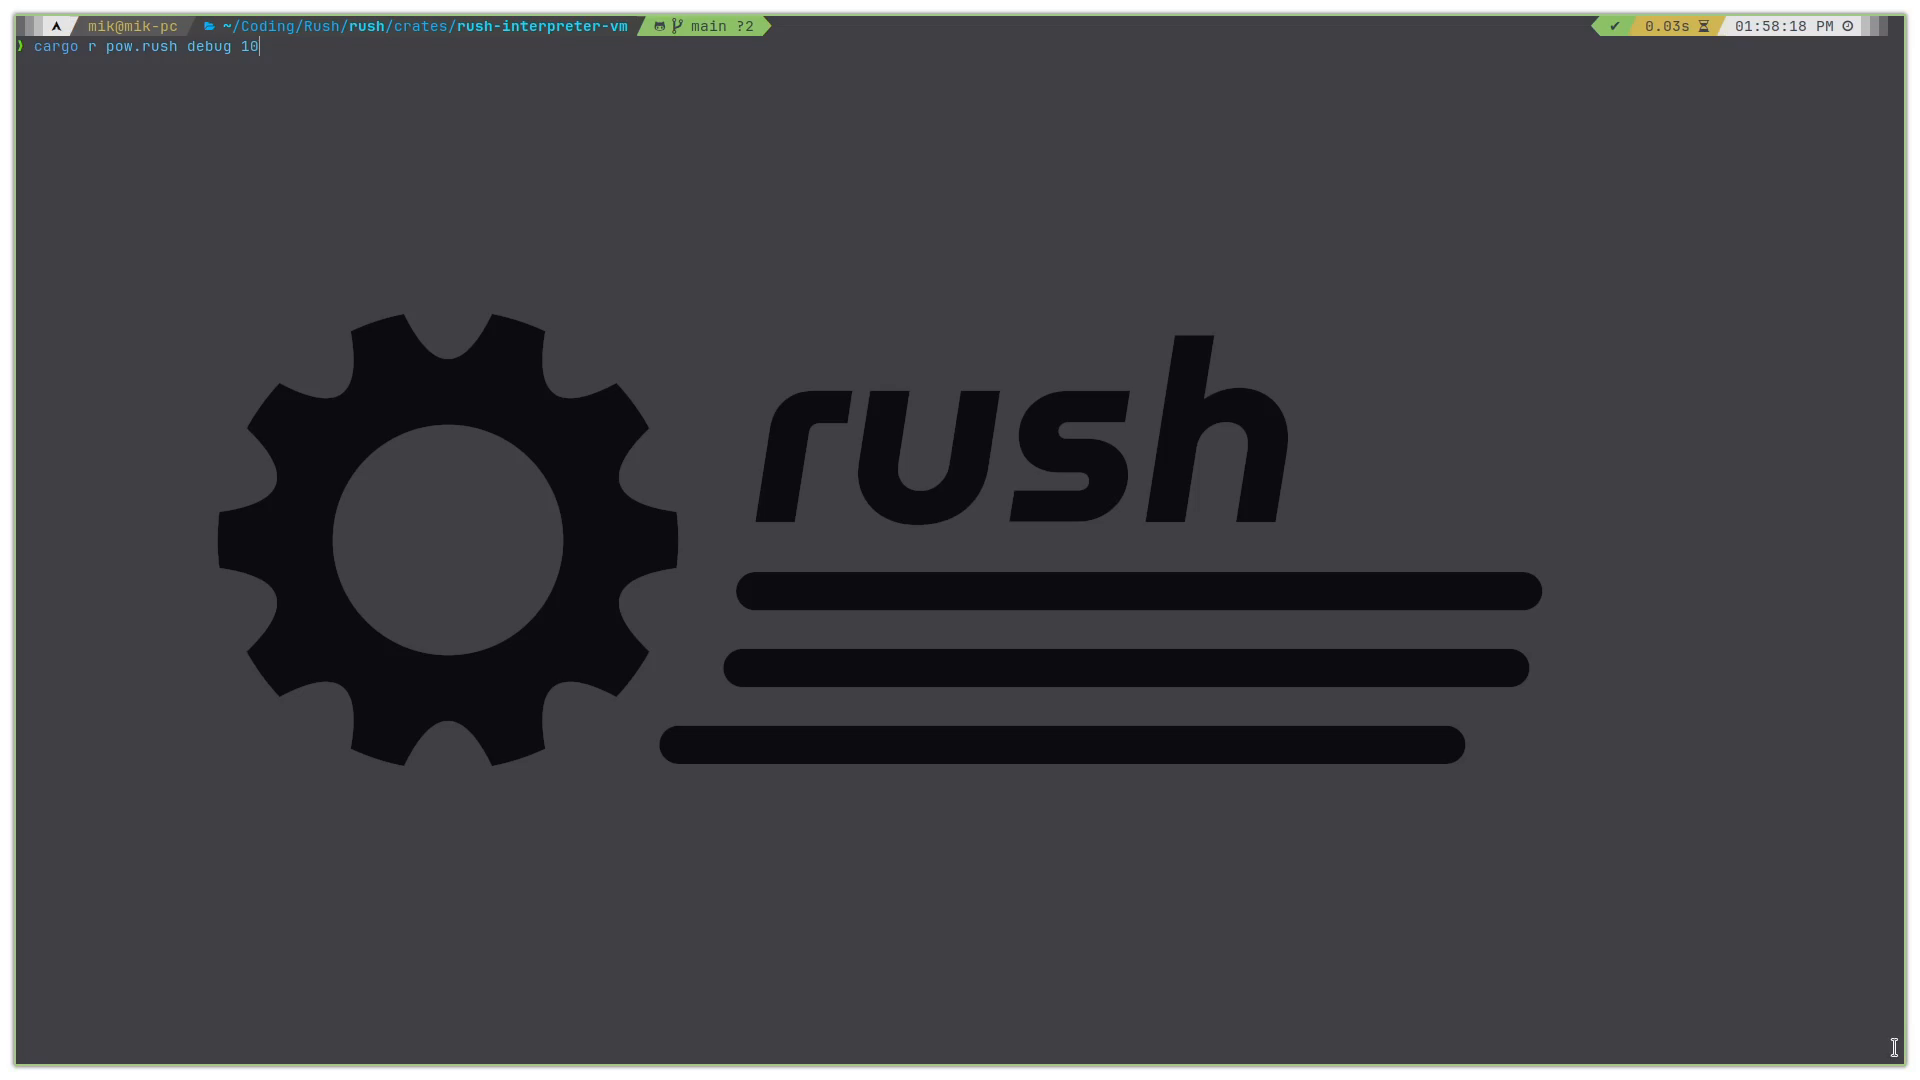
\includegraphics[width=.95\textwidth]{assets/01_rush_presentation_vm.png}}{assets/01_rush_presentation_vm.mkv}
		}
	\end{figure}
\end{frame}

\begin{frame}{VM: Fazit}
	\begin{itemize}
		\item Ca. 2.7 mal schneller als der Tree-walking Interpreter
		\item Einfache Implementierung des Compilers
		      \begin{itemize}
			      \item  Stack-basierte Architektur
			      \item Gleichzeitige Entwicklung von VM und Compiler
			      \item Hoher Abstraktionsgrad
		      \end{itemize}
	\end{itemize}
\end{frame}
